\section{Atividades}

\subsection{Atividade 1 -- Scan de Portas}

\begin{figure}[H]
    \centering
    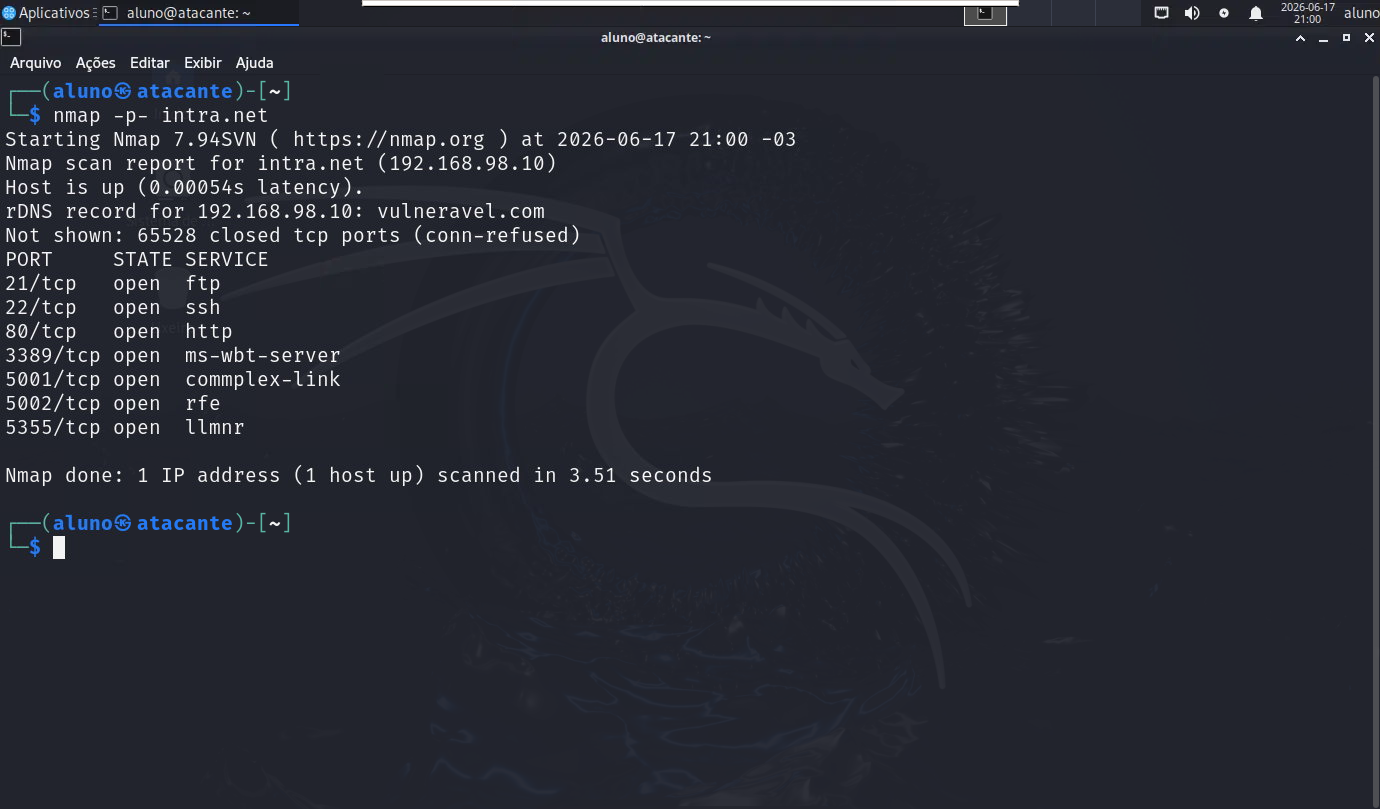
\includegraphics[width=0.95\textwidth]{./fig/atividade1-nmap.png}
    \caption{Varredura de portas utilizando Nmap.}
\end{figure}

\paragraph{}
Foi realizada uma varredura completa das portas TCP do alvo utilizando o Nmap.
O objetivo foi identificar quais serviços estavam acessíveis e quais portas
encontravam-se abertas para futuras etapas de enumeração.

\subsection{Atividade 2 -- Enumeração de Versões}

\begin{figure}[H]
    \centering
    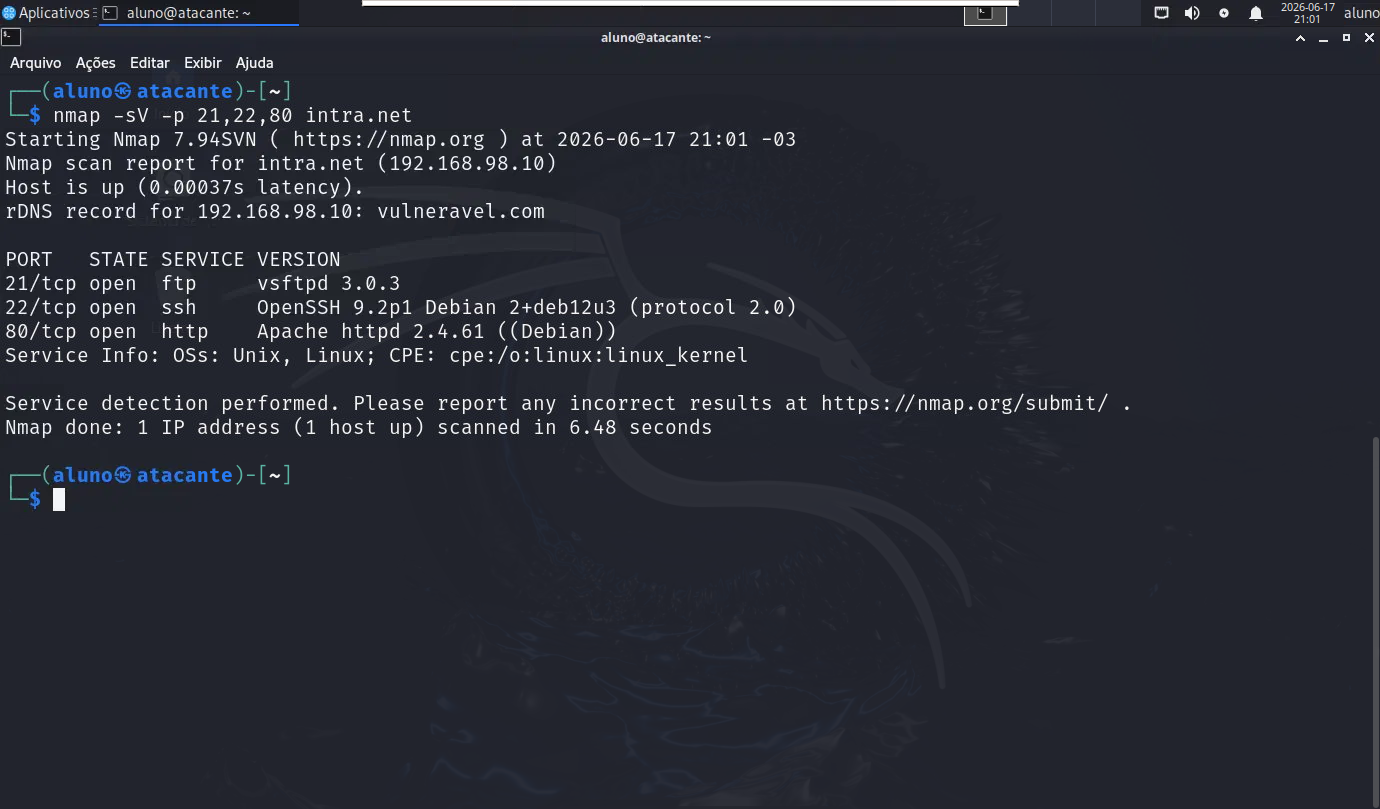
\includegraphics[width=0.95\textwidth]{./fig/atividade2-versoes.png}
    \caption{Identificação das versões dos serviços.}
\end{figure}

\paragraph{}
Utilizando a opção de detecção de versões do Nmap, foram identificadas as
versões dos serviços executados nas portas abertas, permitindo avaliar a
existência de vulnerabilidades conhecidas associadas aos softwares
identificados.

\newpage
\subsection{Atividade 3 -- Banner Grabbing}

\begin{figure}[H]
    \centering
    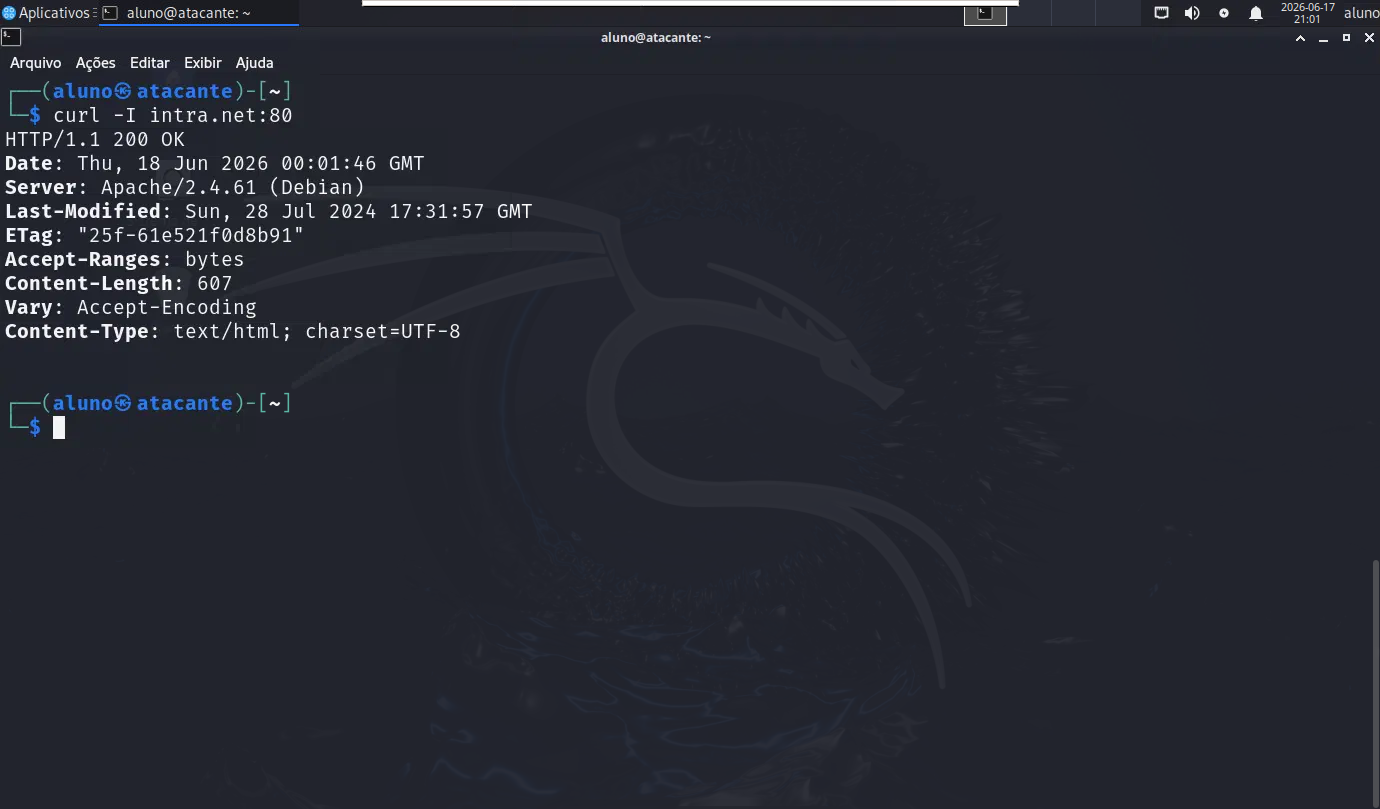
\includegraphics[width=0.95\textwidth]{./fig/atividade3-banner.png}
    \caption{Coleta de banners utilizando cURL.}
\end{figure}

\paragraph{}
Foi realizada a coleta de informações disponibilizadas pelos serviços por meio
dos cabeçalhos HTTP. Essa técnica permitiu identificar detalhes do servidor,
versões de software e outras informações relevantes para a fase de
reconhecimento.

\subsection{Atividade 4 -- Enumeração Web}

\begin{figure}[H]
    \centering
    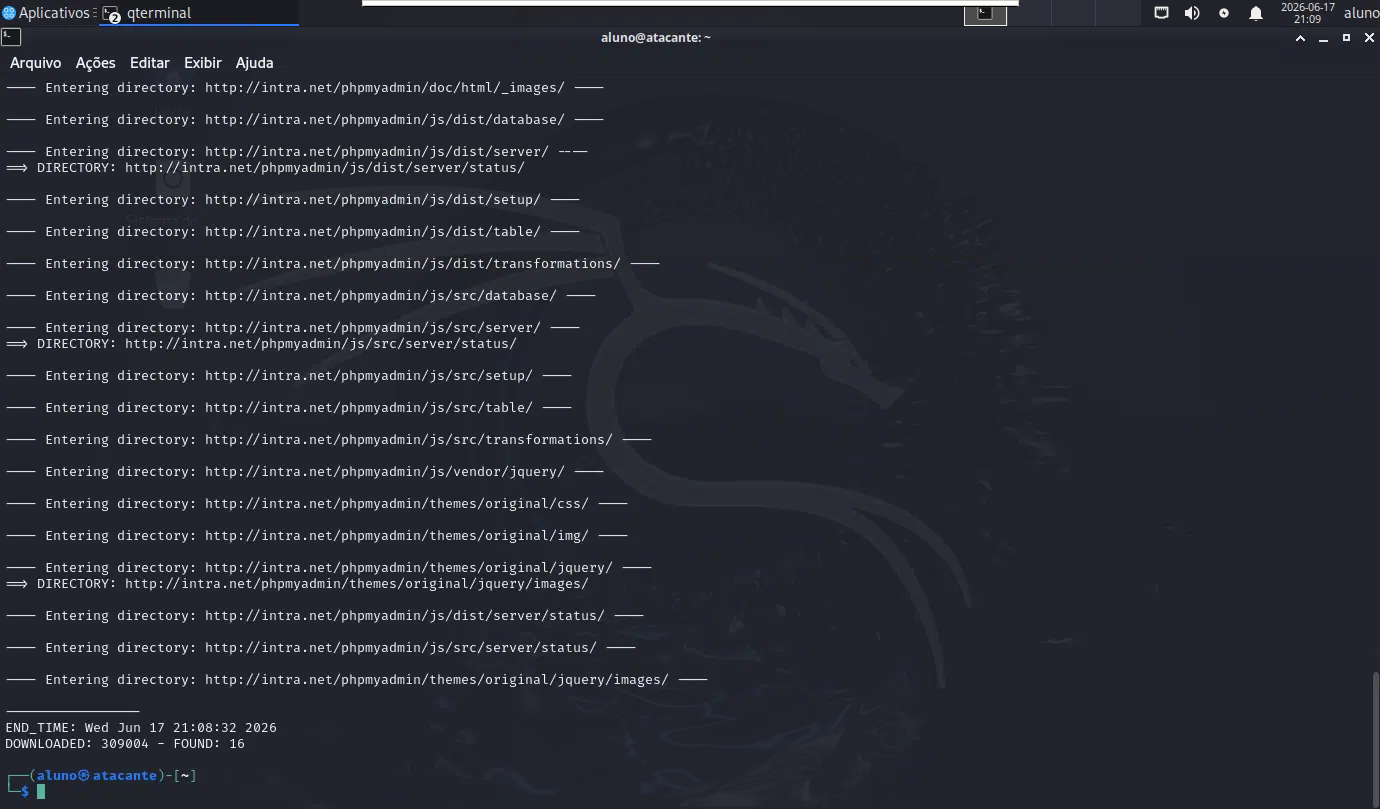
\includegraphics[width=0.95\textwidth]{./fig/atividade4-dirb.png}
    \caption{Enumeração de diretórios utilizando Dirb.}
\end{figure}

\begin{figure}[H]
    \centering
    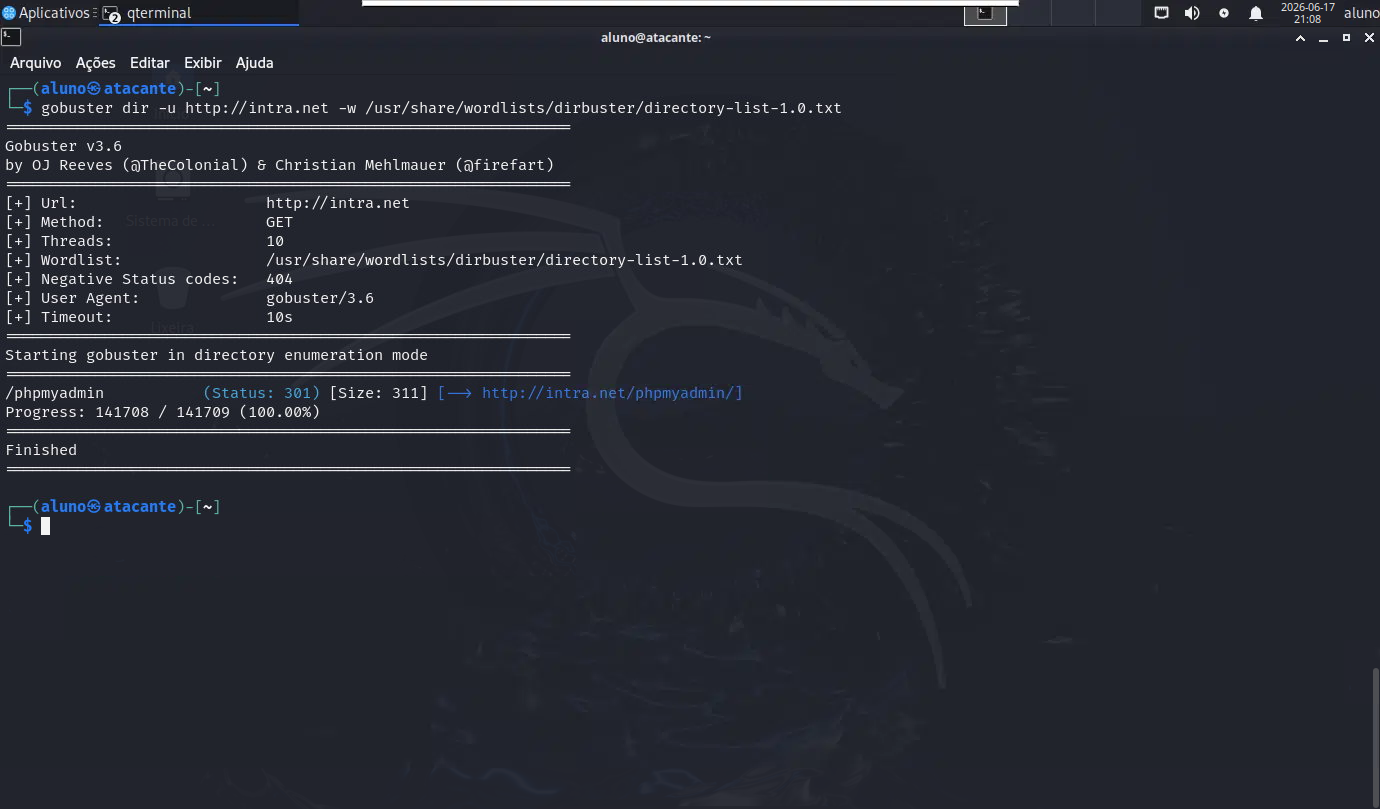
\includegraphics[width=0.95\textwidth]{./fig/atividade4-gobuster.png}
    \caption{Enumeração de diretórios utilizando Gobuster.}
\end{figure}

\begin{figure}[H]
    \centering
    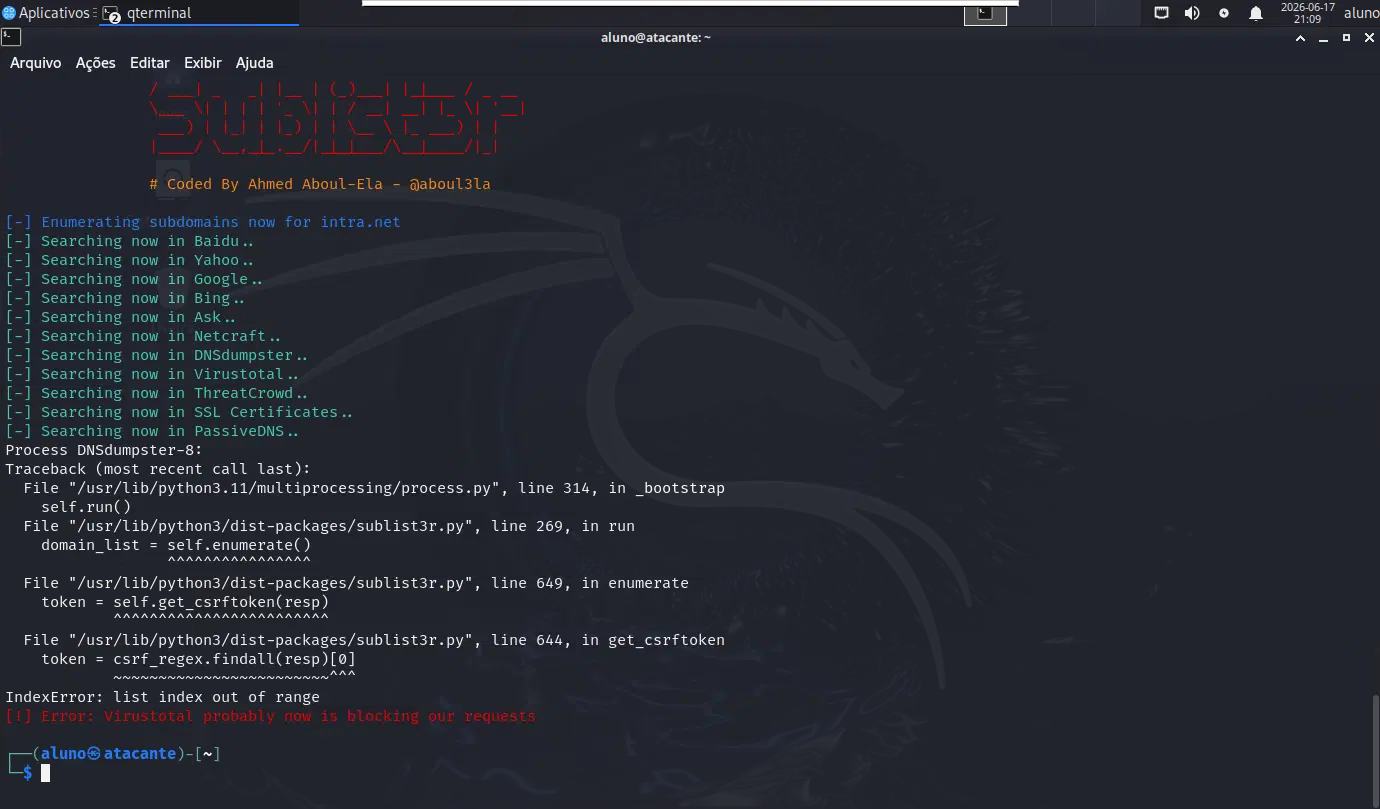
\includegraphics[width=0.95\textwidth]{./fig/atividade4-sublist3r.png}
    \caption{Enumeração de subdomínios utilizando Sublist3r.}
\end{figure}

\paragraph{}
Foram utilizadas ferramentas de enumeração de conteúdo web para identificar
diretórios, arquivos e possíveis subdomínios relacionados ao alvo. Essas
informações auxiliam no mapeamento da superfície de ataque disponível.

\subsection{Atividade 5 -- Scan com Metasploit}

\begin{figure}[H]
    \centering
    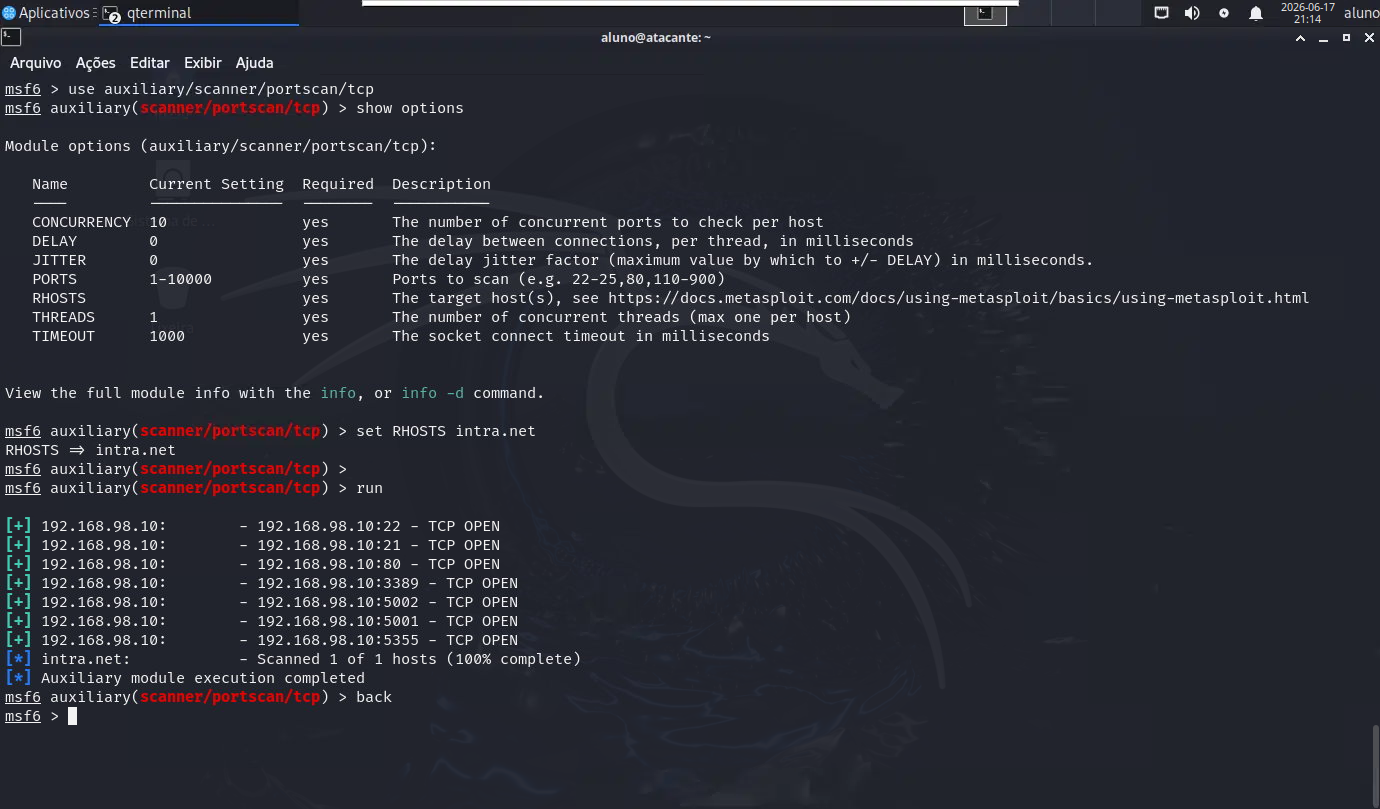
\includegraphics[width=0.95\textwidth]{./fig/atividade5-portscan.png}
    \caption{Varredura de portas utilizando Metasploit.}
\end{figure}

\paragraph{}
Foi utilizado o módulo de port scanning do Metasploit Framework para validar
as portas abertas identificadas anteriormente e familiarizar-se com os
recursos de enumeração da ferramenta.

\newpage
\subsection{Atividade 5.1 -- Enumeração do Serviço SSH}

\begin{figure}[H]
    \centering
    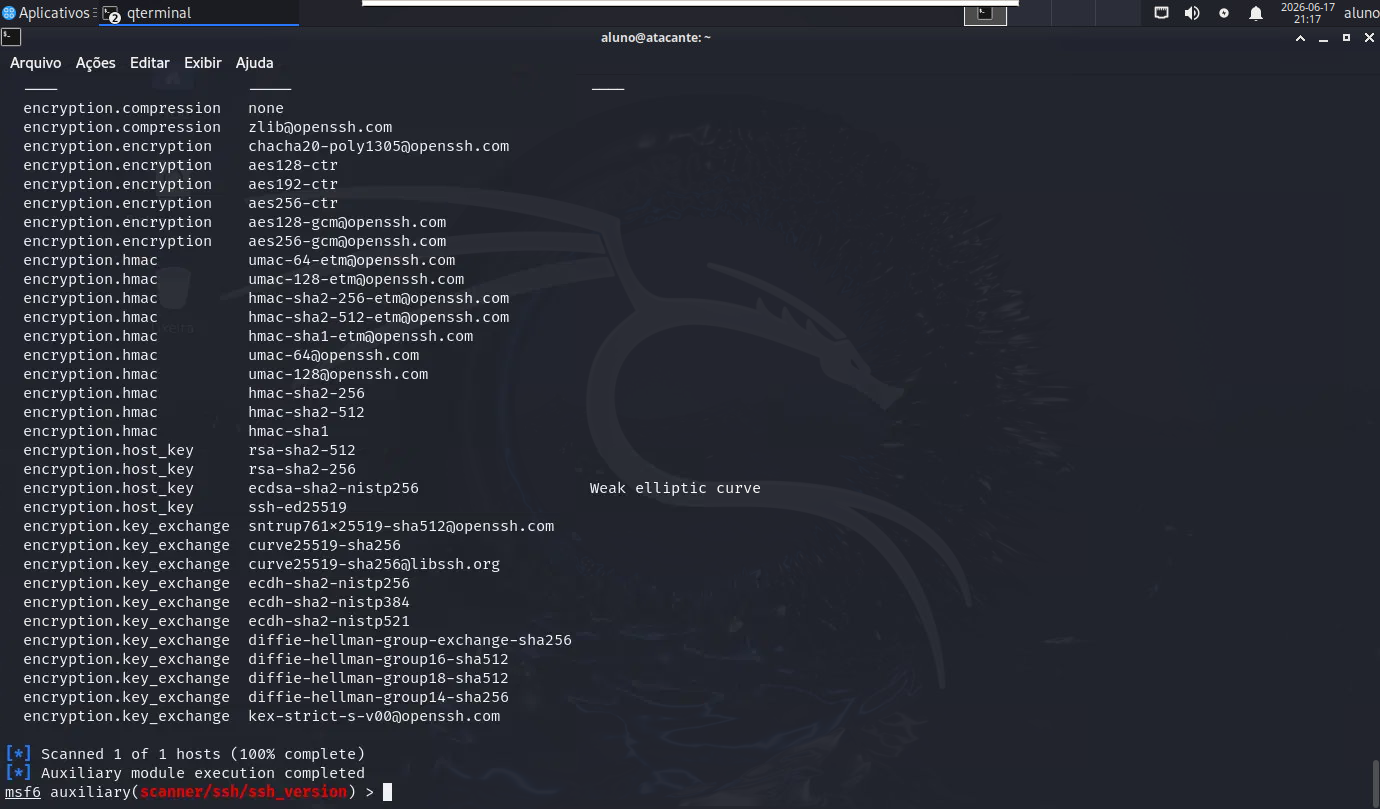
\includegraphics[width=0.95\textwidth]{./fig/atividade5-ssh.png}
    \caption{Identificação da versão do serviço SSH.}
\end{figure}

\paragraph{}
O módulo \texttt{auxiliary/scanner/ssh/ssh\_version} foi utilizado para
coletar o banner do serviço SSH e identificar a versão do software em
execução.

\newpage
\subsection{Atividade 5.2 -- Enumeração do Serviço FTP}

\begin{figure}[H]
    \centering
    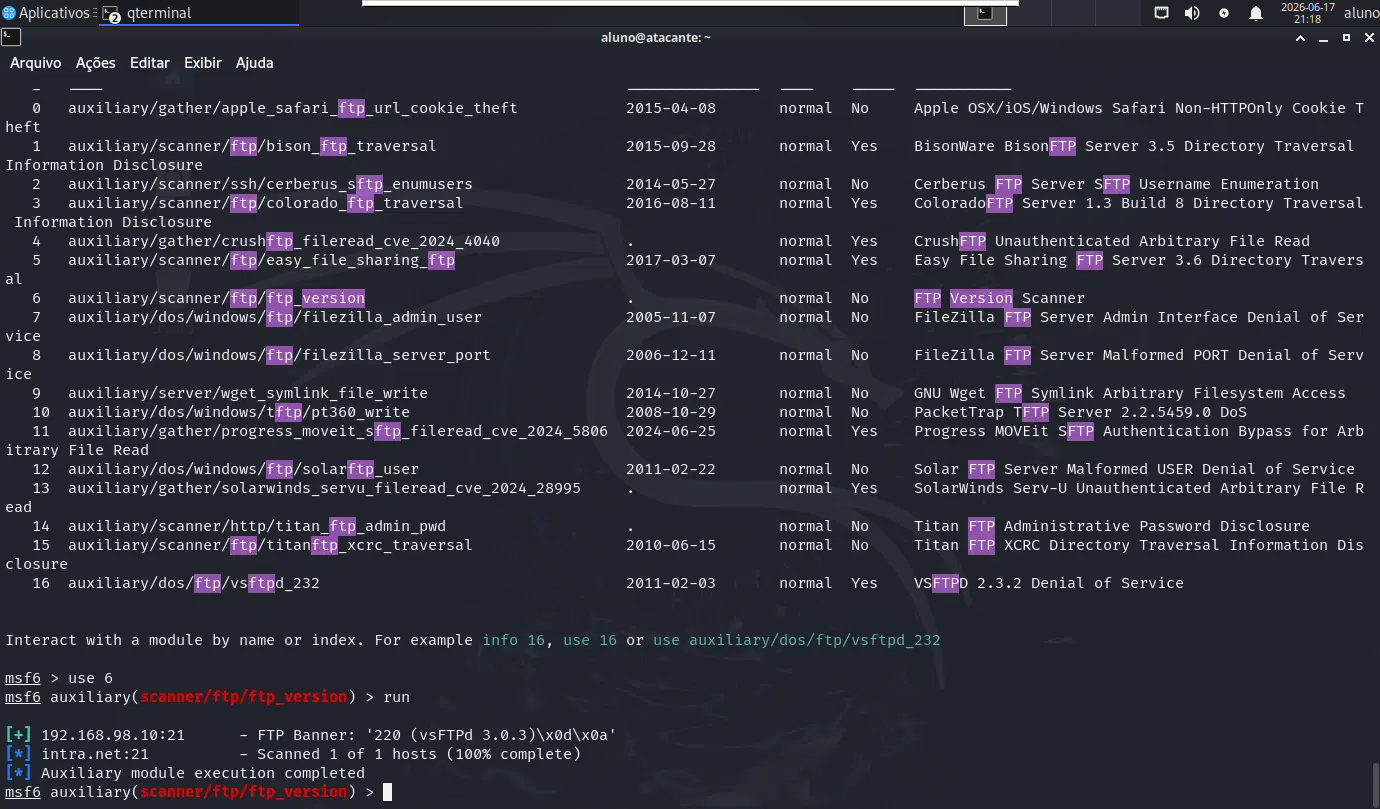
\includegraphics[width=0.95\textwidth]{./fig/atividade5-ftp.png}
    \caption{Identificação da versão do serviço FTP.}
\end{figure}

\paragraph{}
O módulo \texttt{auxiliary/scanner/ftp/ftp\_version} foi utilizado para obter
o banner do serviço FTP e identificar a versão do servidor disponível no
alvo.
